\subsection{Case05 - Broadcast}
\label{P4_ether_case05}

En este caso de uso, se desarrollará un programa p4 que haga Broadcast. En este caso únicamente se hará Broadcast a nivel de enlace, capa 2. La motivación de este caso de uso es ver la diferencia de dificultad respecto del entorno \gls{xdp} donde se tuvo que anclar de manera adicional un \textit{bytecode} e\gls{bpf} en el \gls{tc}, además del propio programa \gls{xdp} anclado en la interfaz para lograr realizar un broadcast.\\
\par

Para conseguir hacer una difusión de los paquetes en P4, se hará uso de los llamados grupos multicast. Los grupos multicast se utilizan para difundir por una serie de números de puertos del ``switch". Para más información sobre de dónde salen estos números de puerto vuelva al case04 (\ref{P4_ether_case04}) donde se explica que representan estos identificadores y cuándo se asignan. Cada grupo multicast tiene un identificador único, y en él se definen una serie de réplicas, es decir, cuántas copias del paquete se llevarán a cabo y qué números de puerto se verán afectados.\\
\par

Los grupos multicast se definen en la información del plano de control del ``switch", bien vía P4Runtime ó vía json con los ficheros \texttt{sX-runtime.json}. A continuación, en el bloque \ref{code:case05_p4_ether_json} se deja la definición del grupo multicast utilizado para este caso de uso.  

\begin{lstlisting}[language= bash, style=Consola, caption={Ejemplo Json Grupo Multicast - Case05},label=code:case05_p4_ether_json]
    "multicast_group_entries" : [
        {
          "multicast_group_id" : 1,
          "replicas" : [
            {
              "egress_port" : 1,
              "instance" : 1
            },
            {
              "egress_port" : 2,
              "instance" : 1
            },
            {
              "egress_port" : 3,
              "instance" : 1
            }
          ]
        }
      ]
\end{lstlisting}
\vspace{0.5cm}

Con esta definición se está indicando que todos los paquetes que pertenezcan al grupo multicast cuyo identificador sea 1, generarán una copia del paquete por los puertos del ``switch" 1, 2 y 3. Es decir por todos los puertos de nuestro ``switch" para este caso de uso. Por tanto la acción de broadcast/multicast será la siguiente:

\begin{lstlisting}[language=C, style=P4-color, caption={Acción propuesta para llevar a cabo el Broadcast - Case05},label=code:case05_p4_ether_prog1]
    action multicast() {
            standard_metadata.mcast_grp = 1;
    }
\end{lstlisting}
\vspace{0.5cm}

Únicamente se asigna el paquete a dicho grupo multicast, y el \gls{bmv2} ya se encarga de clonar el paquete y reenviarlo por los puertos indicados. Dado que no se quiere generar paquetes por el puerto por el cual se recibió el paquete de broadcast, podría plantearse tener tantos grupos multicast como puertos tuviera el \gls{bmv2}, generando copias por puertos específicos y asociando cada grupo multicast a los paquetes que llegaran por cada puerto. Pero esta solución no sería del todo escalable. Por ello, como se puede ver en el grupo multicast (bloque de código \ref{code:case05_p4_ether_json}), se generan copias en todos los puertos asociados a esta instancia del \gls{bmv2}. Será por tanto en la fase de egress cuando se comprueben los metadatos del paquete, y si el puerto de entrada es igual al puerto de salida, se descartará el paquete (Ver bloque de código \ref{code:case05_p4_ether_prog2}).\\
\par

\begin{lstlisting}[language=C, style=P4-color, caption={Acción propuesta para descartar paquetes sobrantes de Broadcast - Case05},label=code:case05_p4_ether_prog2]
    control MyEgress(inout headers hdr,
                 inout metadata meta,
                 inout standard_metadata_t standard_metadata) {
    
        action drop() {
            mark_to_drop(standard_metadata);
        }
    
        apply {
            // Prune multicast packet to ingress port to preventing loop
            if (standard_metadata.egress_port == standard_metadata.ingress_port)
                drop();
        }
}

\end{lstlisting}
\vspace{0.5cm}

En este caso, se ha encontrado que implementar esta funcionalidad en P4 es mucho más sencillo que con \gls{xdp}. Por lo que, en caso de necesitar probar protocolos que implementen la difusión como parte de su lógica, es mucho más recomendable y viable hacer uso de P4.

\vspace{0.5cm}
\textbf{Compilación y puesta en marcha del escenario}\\
\par

Para la compilación del programa P4 se hará uso del compilador P4c (más información sobre el proceso de compilación en la subsección \ref{p4_ether_case01}).\\
\par

Dado que las personas que quieran replicar los casos de uso puede que no estén muy familiarizadas con todo este proceso de compilación y carga en los procesos de \gls{bmv2}, se ha dispuesto un de un Makefile para automatizar las tareas de compilación y carga, y las tareas de limpieza del caso de uso. Entonces para la puesta en marcha del caso de uso se deben seguir los pasos indicados en el bloque \ref{code:case05_p4_ether_load}.

\begin{lstlisting}[language= bash, style=Consola, caption={Compilación programa P4 y puesta en marcha del escenario - Case05},label=code:case05_p4_ether_load]
    # Entramos al directorio 
    cd TFG/src/use_cases/p4/case05

    # Hacemos uso del Makefile
    sudo make run
\end{lstlisting}
\vspace{0.5cm}

Una vez se haya finalizado la comprobación del funcionamiento del caso de uso, se debe hacer uso de otro target (\textit{clean}) del Makefile para limpieza total del directorio según se indica en el bloque \ref{code:case05_p4_ether_unload}.

\begin{lstlisting}[language= bash, style=Consola, caption={Limpieza del escenario P4 - Case05},label=code:case05_p4_ether_unload]
    # Hacemos uso del Makefile
    sudo make clean
\end{lstlisting}
\vspace{0.5cm}

Es importante señalar que este target limpiará tanto los ficheros auxiliares para la carga del programa P4 en el \gls{bmv2}, como los directorios de \texttt{pcaps}, \texttt{log}, y \texttt{build} generados en la puesta en marcha del escenario. Por lo que si se desea conservar las capturas de las distintas interfaces de los distintos \gls{bmv2}, cópielas o haga la limpieza del escenario a mano siguiendo las indicaciones del bloque \ref{code:case05_p4_ether_unload2}.\\
\par

\begin{lstlisting}[language= bash, style=Consola, caption={Limpieza segura del escenario P4 - Case04},label=code:case05_p4_ether_unload2]
    # Limpiamos Mininet
    sudo mn -c
    
    # Limpiamos los directorios generados dinámicamente en la carga del escenario
    sudo rm -rf build logs
\end{lstlisting}


\vspace{0.5cm}
\textbf{Comprobación del funcionamiento}\\
\par
Una vez realizado el make run en el directorio, se tendrá levantada la topología descrita para este caso de uso, la cual se puede apreciar en la figura \ref{fig:case05_p4_ether_scenario}.


% figura escenario
\begin{figure}[ht]
    \centering
    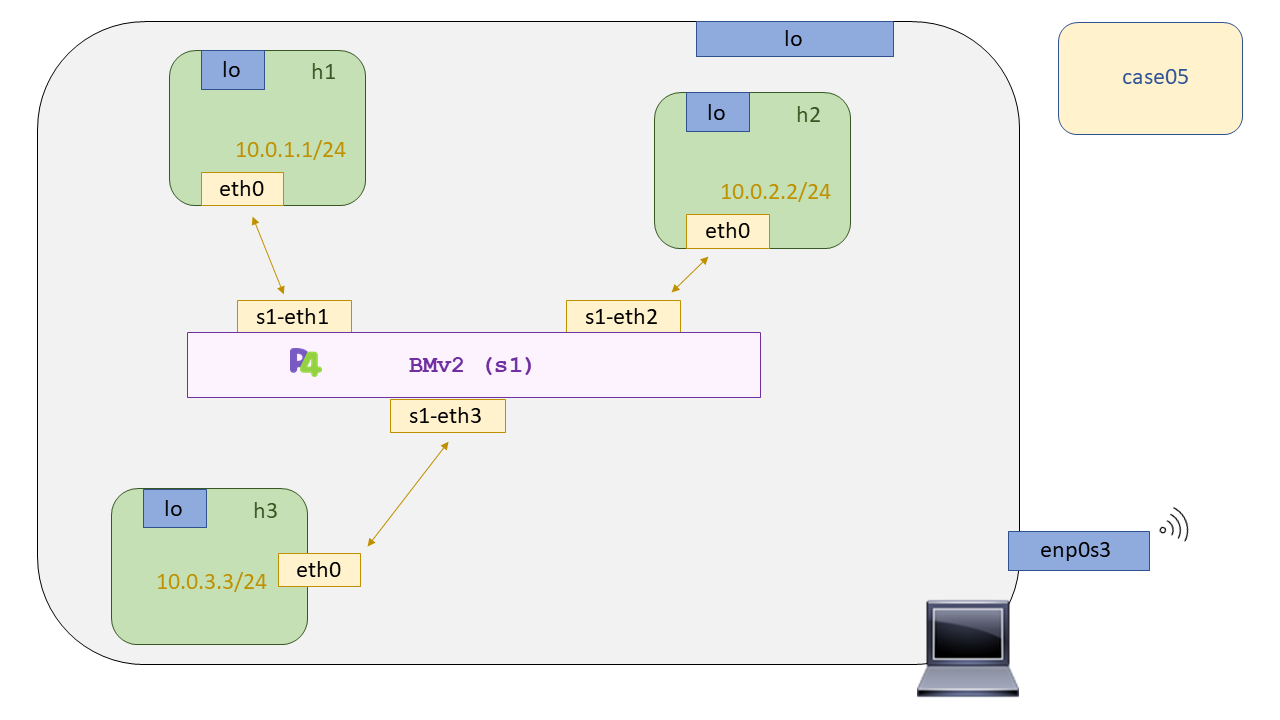
\includegraphics[width=16cm]{archivos/img/dev/p4/case05/scenario.png}
    \caption{Escenario del Case05 - P4}
    \label{fig:case05_p4_ether_scenario}
\end{figure}

Volviendo de nuevo a la comprobación del funcionamiento del caso de uso, se tendrá la CLI de Mininet abierta, por lo que se procederá a abrir tres terminales, una por cada host de la topología. Esto se puede hacer conseguir siguiendo las indicaciones del bloque \ref{code:case05_p4_ether_func1}.

\begin{lstlisting}[language= bash, style=Consola, caption={Apertura de terminales - Case05},label=code:case05_p4_ether_func1]
    mininet> xterm h1 h2 h3 
\end{lstlisting}
\vspace{0.5cm}

Cuando ya se tengan las tres terminales abiertas, se procederá a escuchar las interfaces de los \texttt{host2} y \texttt{host3} con la finalidad de comprobar si realmente los paquetes están siendo clonados por los puertos indicados por el grupo multicast. Se hará uso de la herramienta tcpdump, podríamos utilizar también Wireshark.

\begin{lstlisting}[language= bash, style=Consola, caption={Puesta en escucha - Case05},label=code:case05_p4_ether_func2]
    # Hacemos lo mismo en el host2 y host3
    tcpdump -l
\end{lstlisting}
\vspace{1cm}

Una vez que se tenga tcmdump escuchando desde el \texttt{host2} y \texttt{host3}, se va a generar ARP-Request desde el \texttt{host1} para que así, al ir con MAC destino en difusión se propague por todos los posibles puertos del ``switch" menos por aquel por el cual le llegó. Por tanto, para generar dicho ARP-Request se seguirán los pasos del bloque \ref{code:case05_p4_ether_func3}.

\begin{lstlisting}[language= bash, style=Consola, caption={Generación de ARP-Request - Case05},label=code:case05_p4_ether_func3]
    # Desde el host1
    arping 10.0.2.2
\end{lstlisting}
\vspace{1cm}

Como se puede apreciar en la figura \ref{fig:case05_p4_ether_func1}, el caso de uso funciona correctamente. Se puede observar cómo el paquete ARP-Request está llegando tanto al \texttt{host2} como al \texttt{host3}. Pero solo será el \texttt{host2}, en este caso, el que contesta ya que va dirigido a éste. Se puede ver que al \texttt{host3} solo le llega un ARP-Request, y después se detiene.\\
\par
Esto es así ya que al completarse la resolución ARP el \texttt{host1} ya conoce la dirección MAC del \texttt{host2}, por tanto los ARP-Request que se generen a posteriori llevarán la MAC destino la del \texttt{host2}, entonces el ``switch" no lo difundirá por todos su puertos, se lo pasará directamente al \texttt{host2}.\\
\par

\newpage

\begin{figure}[h!]
    \centering
    \begin{subfigure}[b]{\textwidth}
    	\centering
        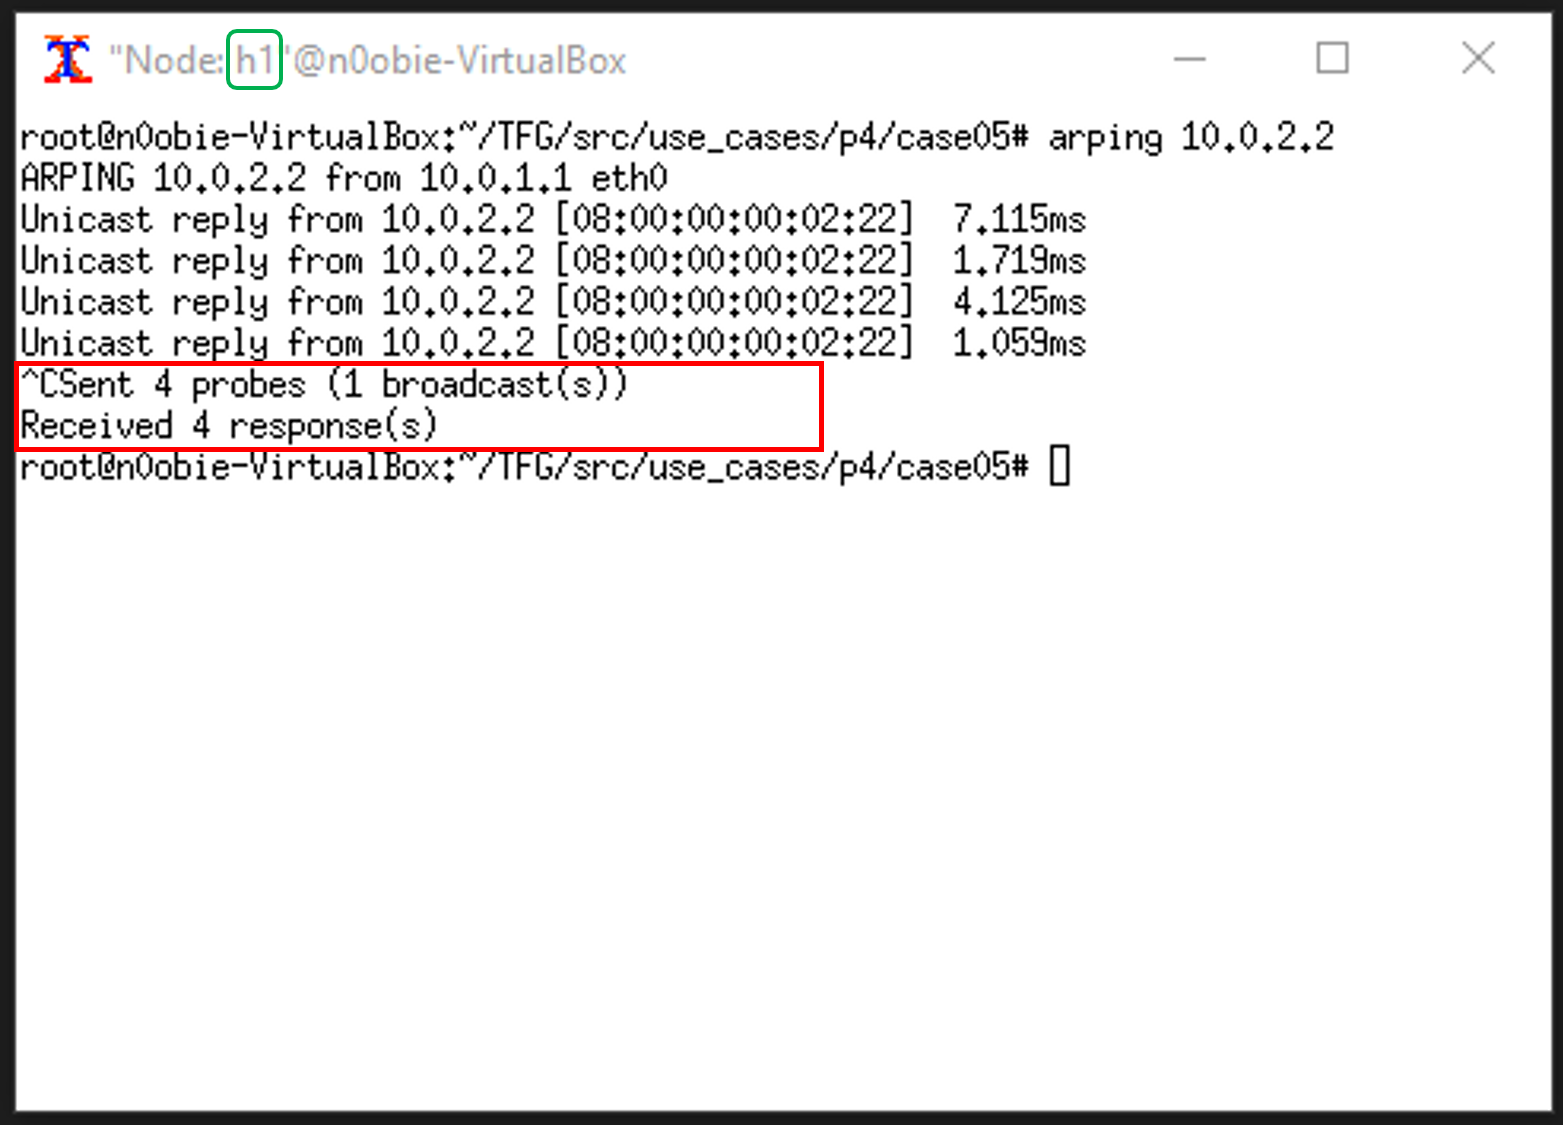
\includegraphics[width=8.2cm]{archivos/img/dev/p4/case05/demo_case05_1_edited.png}
        \caption{Ejecución de arping en el Host1 hacia el Host2}
        \label{fig:case05_p4_ether_func_ping}
    \end{subfigure}
    \par\bigskip
    \begin{subfigure}[b]{\textwidth}
    	\centering
        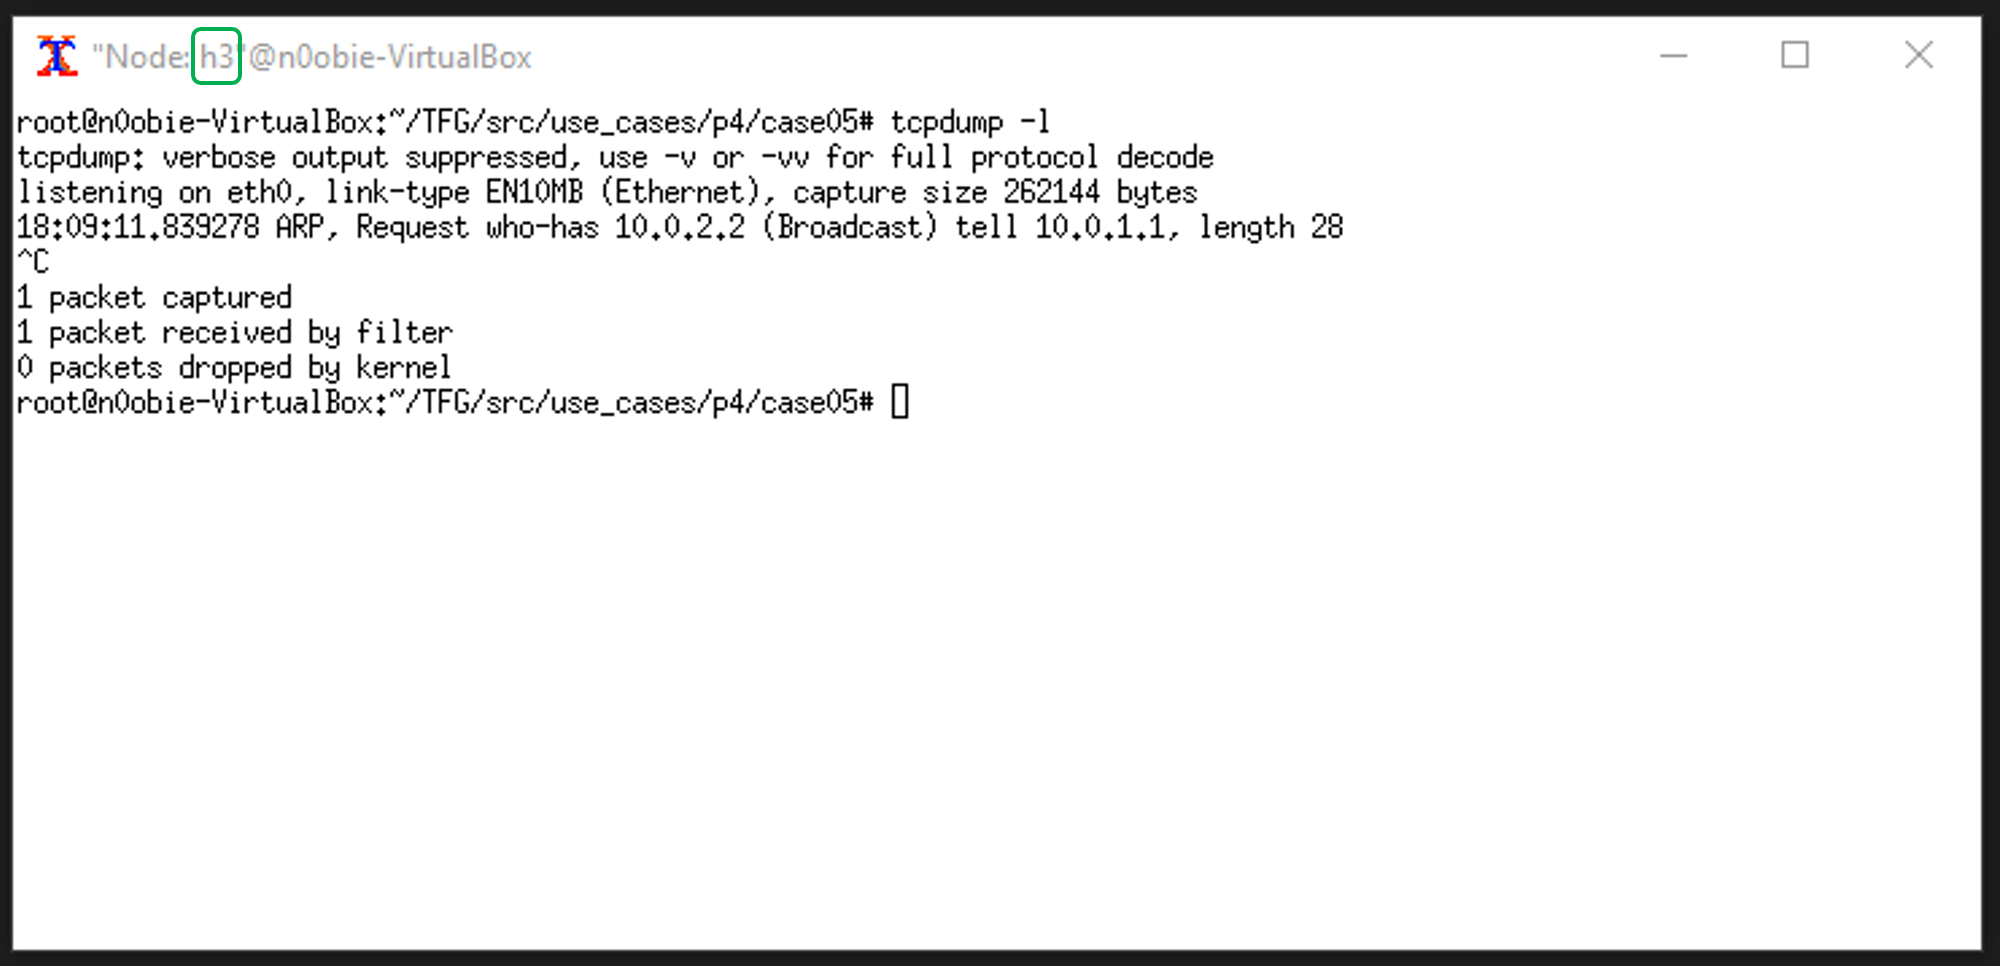
\includegraphics[width=12cm]{archivos/img/dev/p4/case05/demo_case05_2_edited.png}
        \caption{Escucha con Tcpdump en el Host3}
        \label{fig:case05_p4_ether_func_list1}
    \end{subfigure}
    \par\bigskip
    \begin{subfigure}[b]{\textwidth}
    	\centering
        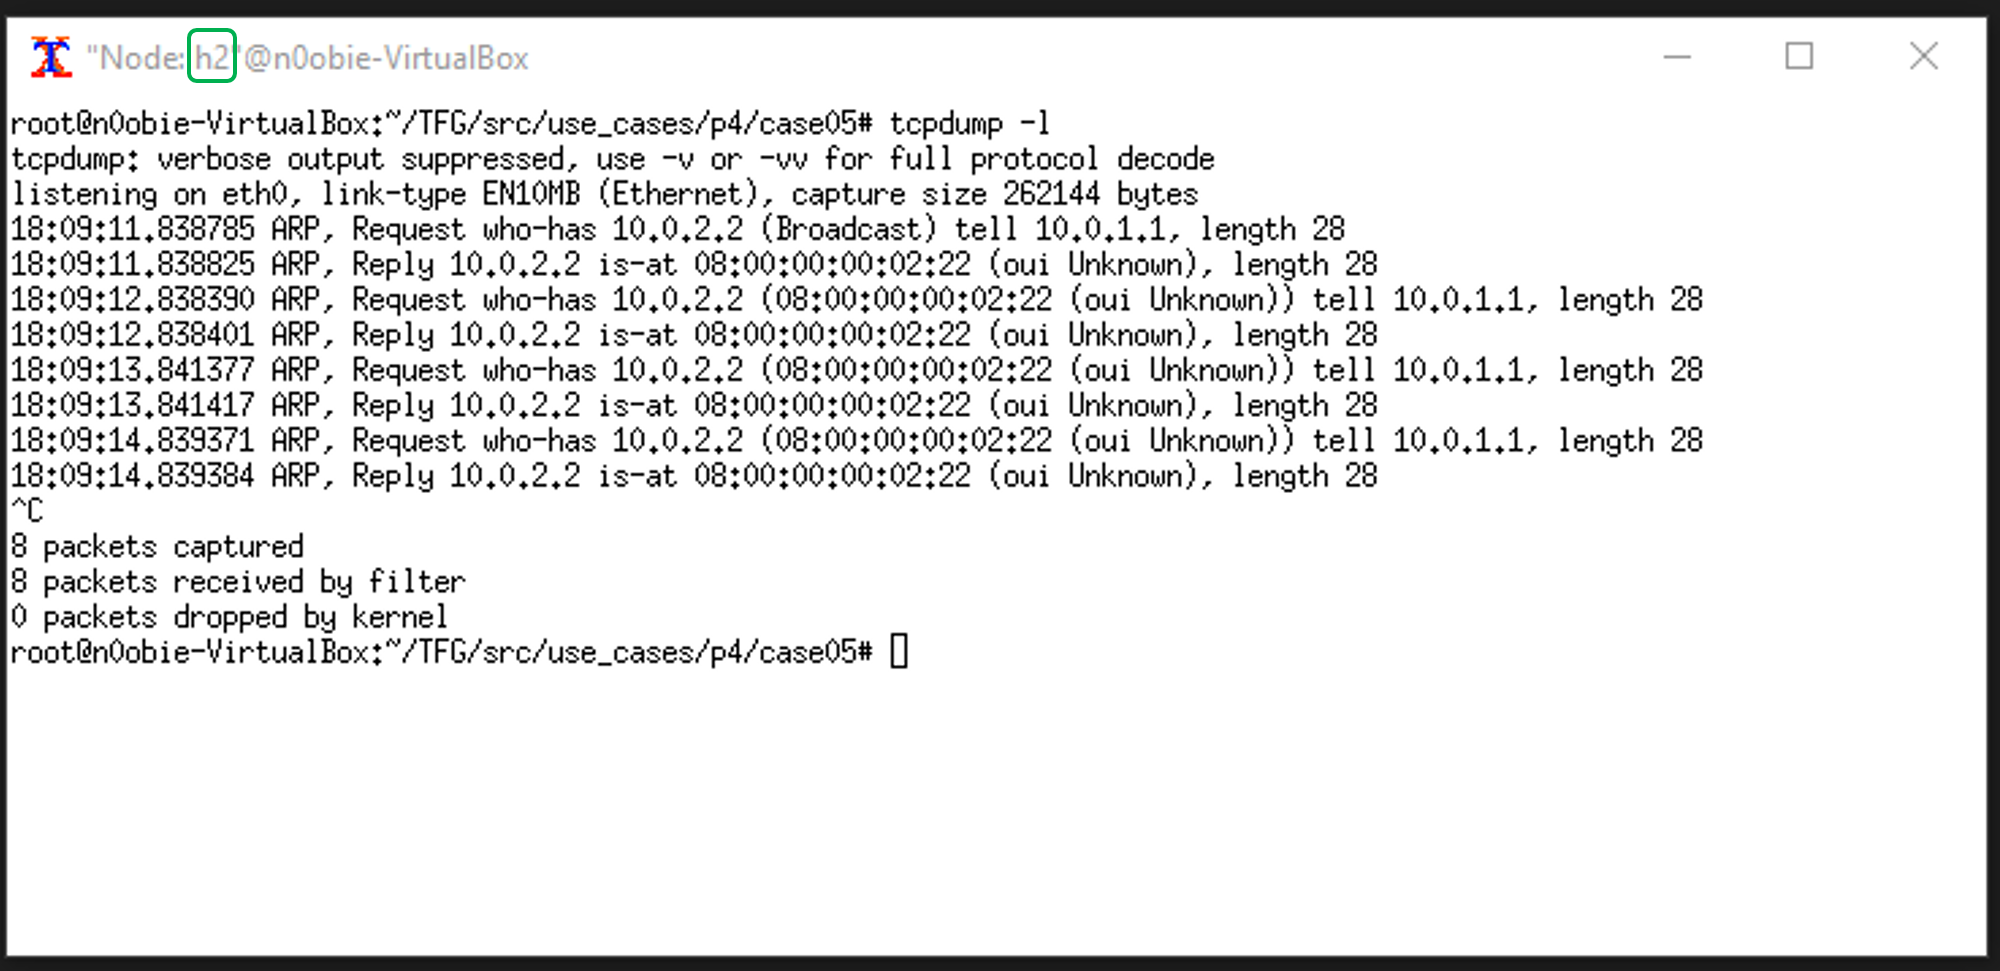
\includegraphics[width=12cm]{archivos/img/dev/p4/case05/demo_case05_3_edited.png}
        \caption{Escucha con Tcpdump en el Host2}
        \label{fig:case05_p4_ether_func_list2}
    \end{subfigure}
    
    \caption{Comprobación de funcionamiento del Case05 - P4}
    \label{fig:case05_p4_ether_func1}
\end{figure}

\newpage
